\subsection{Sztuczna inteligencja przyjaznych jednostek.}

Kontrola jednostek przez gracza odbywa się za pomocą wybory jednej z opcji w dwóch fazach
\begin{itemize}
\item Faza wybrania jednostek
  \begin{itemize}
    \item Wszyscy
    \item Jednostki bliskozasięgowe 
    \item Jednostki hybrydowe
    \item Jednostki dalekozasięgowe
    \item Opcja anulowania wyboru
  \end{itemize}

\item Faza wydania rozkazu
  \begin{itemize}
    \item Podążanie za graczem
    \item Zatrzymanie
    \item Atak
    \item Podejście do wskazanego przez gracza miejsca
    \item Ucieczka
      \item Opcja anulowania rozkazu
  \end{itemize}
\end{itemize}

Wydanie rozkazu polega na kliknięciu przycisku odpowiedzialnego za wejście w tryb wydawania poleceń, a następnie
wybraniu numeru opcji reprezentującej grupę jednostek, której komenda ma dotyczyć. Ostatecznie należy podać numer rozkazu, który zostanie wydany.
Przykładowa reprezentacja graficzna systemu jest widoczna na rysunku \ref{fig:mnb}.
Wykorzystanie tego modelu pozwala na łatwe rozwinięcie systemu o dodanie nowych metod wyboru grup jednostek oraz możliwych instrukcji dla przyjaznych agentów.

\begin{figure}[h]
\centering
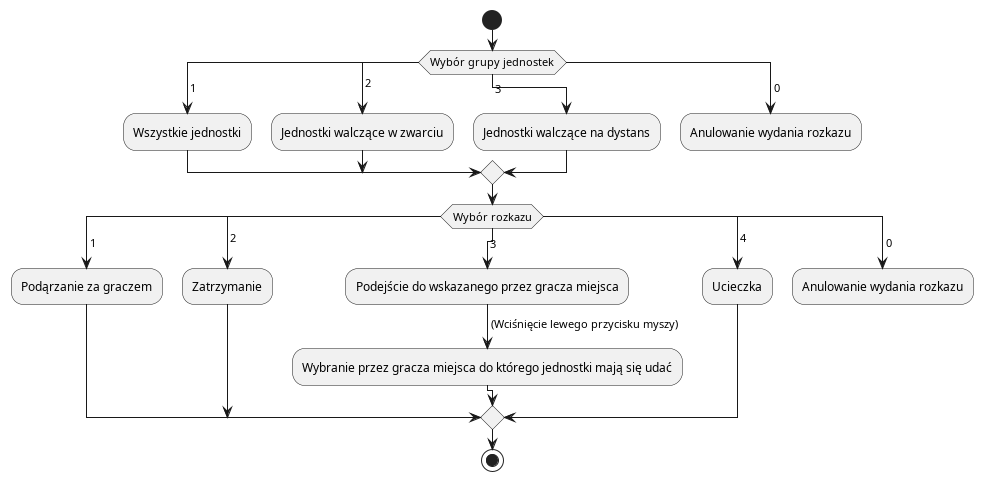
\includegraphics[width=0.6\textwidth]{uml/commands}
\caption{Wizualizacja przepływu sterowania podczas wydawania poleceń jednostkom.}
\end{figure}
